\documentclass[11pt]{article}
\usepackage[hmargin=1in,vmargin=1in]{geometry}
\usepackage{xcolor}
\usepackage{amsmath,amssymb,amsfonts,url,sectsty,framed,tcolorbox,framed,graphicx}
\newcommand{\pf}{{\bf Proof: }}
\newtheorem{theorem}{Theorem}
\newtheorem{lemma}{Lemma}
\newtheorem{proposition}{Proposition}
\newtheorem{definition}{Definition}
\newtheorem{remark}{Remark}
\newcommand{\qed}{\hfill \rule{2mm}{2mm}}

\begin{document}
\noindent
\rule{\textwidth}{1pt}
\begin{center}
{\bf [CS304] Introduction to Cryptography and Network Security}
\end{center}
Course Instructor: Dr. Dibyendu Roy \hfill Winter 2022-2023\\
Scribed by: Srushti Rathva (202051183) \hfill Lecture (Week 3)
\\
\rule{\textwidth}{1pt}

%write here
\section*{One Time Padding (OTP)}
OTP provides perfect secrecy under some conditions. \\ \\
\textbf{Encryption} \\
$ P \rightarrow$ Plaintext \\
$ K \rightarrow$ Secret Key \\
$ E(P,K) \rightarrow P \oplus K = C$ \\ \\
\textbf{Decryption} \\
$ C \rightarrow$ Ciphertext \\
$ K \rightarrow$ Secret Key \\
$ D(C,K) \rightarrow C \oplus K = P$ \\ \\
\textbf{Conditions}\\
1. The secret key $K$ can not be used to encrypt two messages \\
2. length($K$) $\geq$ length($P$) \\
3. $K$ is uniformly selected from the key space \\

\section*{Data Encryption Standard (DES)}
DES is a Feistel cipher which processes plaintext blocks of n = 64 bits, producing 64-bit ciphertext blocks. The effective size of the secret key K is k = 56 bits; more precisely, the input key K is specified as a 64-bit key, 8 bits of which (bits 8, 16,...,64) may be used as parity bits.\\ 

\subsection*{Round Funtion of DES}
The round function of des applies to 48-bit key and the rightmost 32 bits($R_{i-1}$) from the previous round text to produce a 32-bit output. This function is made up of four sections: an expansion function E, a whitener (XOR that adds key), a substitution function S, and a permutation function P.\\
\[ f : \{0, 1\}^{32} \ast \{0, 1\}^{48} \to \{0, 1\}^{32} \]
\[ f(R_{i-1}, K_i) = P(S(E(R_{i-1}) \bigoplus K_i)) \]
\begin{center}
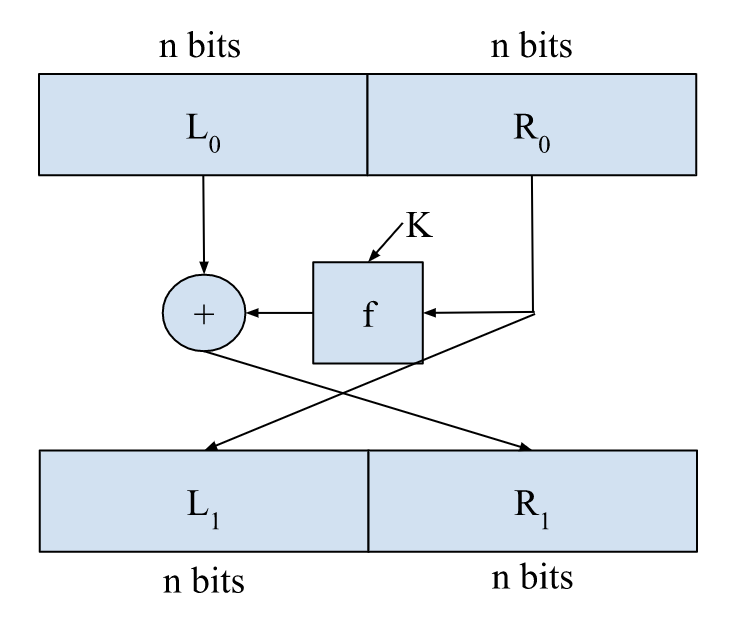
\includegraphics[width=200pt]{p1.png}
\end{center}

\subsubsection*{Expansion Function(E)}
E is a fixed expansion permutation mapping on $R_{i-1}$. Since $R_{i-1}$ is a 32-bit input and $K_i$ is a 48-bit key, we need to expand $R_{i-1}$ to 48 bits. $R_{i-1}$ is divided into 8 4-bit sections. Each 4-bit section is then expanded to 6 bits. This expansion permutation follows a predetermined rule. For each section, input bits 1, 2, 3, and 4 are copied to output bits 2, 3, 4, and 5, respectively. Output bit 1 comes from bit 4 of the previous section; output bit 6 comes from bit 1 of the next section. For easy understanding the expansion can be done using the expansion Table 1.
\[ E : \{0, 1\}^{32} \to \{0, 1\}^{48} \]
Let \hspace{1cm} $R_{i-1}$ = $x_1$$x_2$$x_3$.............$x_{31}$$x_{32}$ \\
So, \hspace{1cm} E($x_1$$x_2$$x_3$.............$x_{31}$$x_{32}$) = $x_{32}$$x_1$$x_2$.............$x_{18}$$x_{19}$.............$x_{31}$$x_{32}$$x_1$ 
\begin{center}
\begin{tabular}{ | c | c | c | c | c | c |}
  \hline
    32&	1&	2&	3&	4&  5\\
    4&	5&	6&	7&	8&  9\\
    8&	9&	10&	11&	12&  13\\
    12&	13&	14&	15&	16&  17\\
    16&	17&	18&	19&	20&  21\\
    20&	21&	22&	23&	24&  25\\
    24&	25&	26&	27&	28&  29\\
    28&	29&	30&	31&	32&  1\\
  \hline
\end{tabular}
\end{center}
\begin{center}
Table 1. Expansion Function Table
\end{center}
\begin{center}
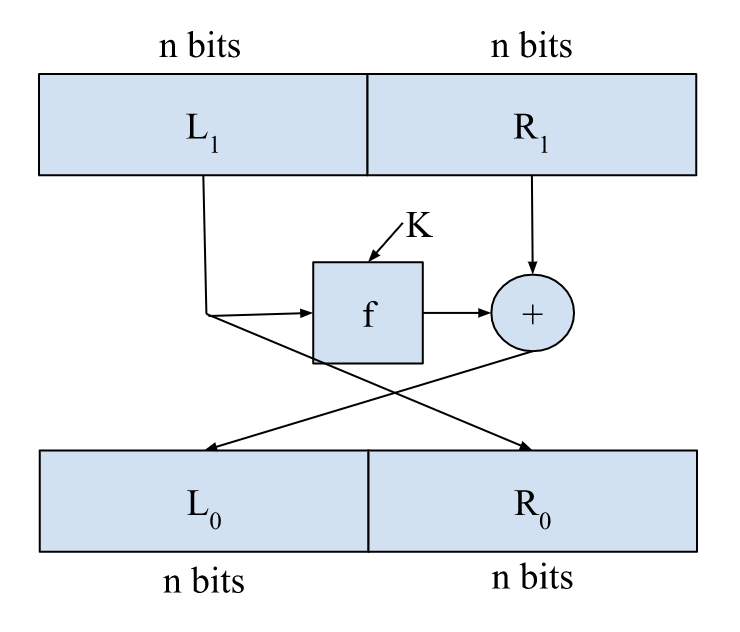
\includegraphics[width=200pt]{p2.png}
\end{center}

\subsubsection*{Whitener (XOR)}
After the expansion function, DES uses the XOR operation on the expanded right section($R_{i-1}$) and the round key($K_i$). Note that both the right section and the round key are 48-bits in length. Also note that the round key is used only in this operation.
\[ Y_i = E(R_{i-1}) \bigoplus K_{i} \]

\subsubsection*{Subtitusion Function(S)}
DES uses 8 S-boxes, each with a 6-bit input and a 4-bit output. The 48-bit data($Y_i$) from the second operation is divided into eight 6-bit chunks, and each chunk is fed into a box.
\[ Y_i = B_0 || B_1 || B_2 || B_3 || B_4 || B_5 || B_6 || B_7 || B_8 \hspace{1cm} len(B_i)=6bits \]
The result of each box is a 4-bit chunk; when these are combined the result is a 32-bit text. The substitution in each box follows a pre-determined rule based on a 4-row by 16-column table. The combination of bits 1 and 6 of the input defines one of four rows; the combination of bits 2 through 5 defines one of the sixteen columns. Because each S-box has its own table, we need eight tables, as shown in Tables 2 to 9.
\[ S(Y_i) = S_0(B_0) || S_2(B_2) || S_3(B_3) || S_4(B_4) || S_5(B_5) || S_6(B_6) || S_7(B_7) || S_8(B_8)\]
\[S_i : \{0, 1\}^{6} \to \{0, 1\}^{4}\]
\[B_i = b_1b_2b_3b_4b_5b_5b_6\]
\[Row(r) = b_1b_6 \hspace{1cm} 0\leq i \leq3 \]
\[Column(c) = b_2b_3b_4b_5b_5 \hspace{1cm} 0\leq i \leq15 \]
\[S_i = Sbox[r][c]\]
\begin{center}
\begin{tabular}{ | c | c | c | c | c | c | c | c | c | c | c | c | c | c | c | c |}
  \hline
    14&	4& 13& 1& 2& 15& 11& 8&	3& 10& 6& 12& 5& 9&	0& 7\\
    0&	15& 7& 4& 14& 2& 13& 10& 3& 6& 12& 11& 9& 5& 3& 8\\
    4&	1& 14& 8& 13& 6& 2& 11&	15& 12& 9& 7& 3& 10& 5& 0\\
    15&	12& 8& 2& 4& 9& 1& 7& 5& 11& 3& 14& 10& 0&	6& 13\\
  \hline
\end{tabular}
\end{center}
\begin{center}
Table 2. S-box 1
\end{center}

\begin{center}
\begin{tabular}{ | c | c | c | c | c | c | c | c | c | c | c | c | c | c | c | c |}
  \hline
    15&	1& 8& 14& 6& 11& 3& 4& 9& 7& 2& 13& 12& 0&	5& 10\\
    3& 13& 4& 7& 15& 2& 8& 14& 12& 0& 1& 10& 6& 9&	11& 5\\
    0& 14& 7& 11& 10& 4& 13& 1& 5& 8& 12& 6& 9& 3&	2& 15\\
    13&	8& 10& 1& 3& 15& 4& 2& 11& 6& 7& 12& 0& 5&	14& 9\\
  \hline
\end{tabular}
\end{center}
\begin{center}
Table 3. S-box 2
\end{center}

\begin{center}
\begin{tabular}{ | c | c | c | c | c | c | c | c | c | c | c | c | c | c | c | c |}
  \hline
    10&	0& 9& 14& 6& 3& 15& 5& 1& 13& 12& 7& 11& 4&	2& 8\\
    13&	7& 0& 9& 3& 4& 6& 10& 2& 8& 5& 14& 12& 11& 15& 1\\
    13&	6& 4& 9& 8& 15& 3& 0& 11& 1& 2& 12& 5&	10& 14& 7\\
    1& 10& 13& 0& 6& 9& 8& 7& 4& 15& 14& 3& 11& 5& 2& 12\\
  \hline
\end{tabular}
\end{center}
\begin{center}
Table 4. S-box 3
\end{center}

\begin{center}
\begin{tabular}{ | c | c | c | c | c | c | c | c | c | c | c | c | c | c | c | c |}
  \hline
    7&	13& 14& 3& 0& 6& 9& 10&	1& 2& 8& 5& 11& 12&	4& 15\\
    13&	8& 11& 5& 6& 15& 0& 3& 4& 7& 2& 12& 1& 10& 14& 9\\
    10&	6& 9& 0& 12& 11& 7&	13& 15& 1& 3& 14& 5& 2& 8& 4\\
    3&	15& 10& 6& 10& 1& 13& 8& 9& 14& 5& 11& 12& 7& 2& 14\\
  \hline
\end{tabular}
\end{center}
\begin{center}
Table 5. S-box 4
\end{center}

\begin{center}
\begin{tabular}{ | c | c | c | c | c | c | c | c | c | c | c | c | c | c | c | c |}
  \hline
    2&	12& 4& 1& 7& 10& 11& 6& 8& 5& 3& 15& 13& 0& 14& 9\\
    14&	11& 2& 12& 4& 7& 13& 1&	5& 0& 15& 10& 3& 9&	8& 6\\
    4&	2& 1& 11& 10& 13& 7& 8& 15& 9& 12& 5& 6& 3& 0& 14\\
    11&	18& 12& 7& 1& 14& 2& 13& 6& 15& 0& 9& 10& 4& 5& 3\\
  \hline
\end{tabular}
\end{center}
\begin{center}
Table 6. S-box 5
\end{center}

\begin{center}
\begin{tabular}{ | c | c | c | c | c | c | c | c | c | c | c | c | c | c | c | c |}
  \hline
    12&	1& 10& 15& 9& 2& 6&	8& 0& 13& 3& 4& 14&	7& 5& 11\\
    10&	15& 4& 2& 7& 12& 9& 5&	6& 1& 13& 14& 0& 11& 3& 8\\
    9&	14& 15& 5& 2& 8& 12& 3& 7& 0& 4& 10& 1& 13& 11& 6\\
    4&	3& 2& 12& 9& 5& 15& 10&	11& 14& 1& 7& 10& 0& 8& 13\\
  \hline
\end{tabular}
\end{center}
\begin{center}
Table 7. S-box 6
\end{center}

\begin{center}
\begin{tabular}{ | c | c | c | c | c | c | c | c | c | c | c | c | c | c | c | c |}
  \hline
    4&	1& 2& 14& 15& 0& 8&	13& 3& 12& 9& 7& 5&	10& 6& 1\\
    13&	0& 11& 7& 4& 9& 1& 10& 14& 3& 5& 12& 2& 15&	8& 6\\
    1&	4& 11& 13& 12& 3& 7& 14& 10& 15& 6& 8& 0& 5& 9& 2\\
    6&	11& 13& 8& 1& 4& 10& 7&	9& 5& 0& 15& 14& 2&	3& 12\\
  \hline
\end{tabular}
\end{center}
\begin{center}
Table 8. S-box 7
\end{center}

\begin{center}
\begin{tabular}{ | c | c | c | c | c | c | c | c | c | c | c | c | c | c | c | c |}
  \hline
    13&	2& 8& 4& 6& 15& 11&	1& 10& 9& 3& 14& 5&	0& 12& 7\\
    1&	15& 13& 8& 10& 3& 7& 4&	12& 5& 6& 11& 10& 14& 9& 2\\
    7&	11& 4& 1& 9& 12& 14& 0& 0& 6& 10& 10& 15& 3& 5& 8\\
    2&	1& 14& 7& 4& 10& 8& 13&	15& 12& 9& 9& 3& 5&	6& 11\\
  \hline
\end{tabular}
\end{center}
\begin{center}
Table 9. S-box 8
\end{center}

\subsubsection*{Permutation Function(P)}
The last operation in the DES function is a permutation with a 32 bit input and a 32-bit output. The input/output relationship for this operation is shown in Table 10 and follows the same general rule as previous tables. For example, the seventh bit of the input becomes the second bit of the output.
\[ P : \{0, 1\}^{32} \to \{0, 1\}^{32} \]
Let $Z_{i}$ be the input of permutation function. \\
\hspace{3cm} $Z_i$ = $x_1$$x_2$$x_3$.............$x_{31}$$x_{32}$ \\
So, \hspace{1cm} P($x_1$$x_2$$x_3$.............$x_{31}$$x_{32}$) = $x_{16}$$x_7$$x_{20}$.............$x_8$$x_{24}$.............$x_{11}$$x_4$$x_{25}$ 
\\
\begin{center}
\begin{tabular}{ | c | c | c | c |}
  \hline
    16&	7&	20&	21\\
    29&	12&	28&	17\\
    1& 15& 23& 26\\
    5&	18&	31&	10\\
    2&	18&	24&	14\\
    32&	27&	3&	9\\
    19&	13&	30&	6\\
    22&	11&	4&	25\\
  \hline
\end{tabular}
\end{center}
\begin{center}
Table 10. Permutation Function Table
\end{center}

\subsection*{Key Scheduling Algorithm}
The round-key generation algorithm generates sixteen 48-bit keys $K_i$ out of a 64-bit secret key K in which 8 extra bits are the parity bits, which are dropped before the actual key-generation. 
\\

The parity drop process drops the parity bits (bits 8, 16, 24, 32, …, 64) from the 64-bit key and permutes the rest of the bits according to the permuted choice 1 table shown in Table 11. The permuted 56 bits key is now assigned to two 28-bit variables $C_0$ and $D_0$.
\[ T = PC_1(K) \]
\[ T = C_0 || D_0 \]
Length($C_0$) = Length($D_0$) = 28bits
\begin{center}
\begin{tabular}{ | c | c | c |c | c | c | c |}
  \hline
    57&	49&	41&	33& 25& 17& 9\\
    1&	58&	50&	42& 24& 26& 18\\
    10&	2&	59&	51& 43& 35& 27\\
    19& 11&	3& 60& 52& 44& 36\\
    &\multicolumn{5}{c}{above for C_0 ; below for D_0}& \hspace{} \\
    63&	55&	47&	39& 31& 23& 15\\
    7&	62&	54&	46& 38& 30& 22\\
    14&	6&	61&	53& 45& 37& 29\\
    21&	13&	5&	28& 20& 12& 4\\
  \hline
\end{tabular}
\end{center}
\begin{center}
Table 11. Permuted Choice 1 Table
\end{center}

The $C_i$ and $D_i$ are generated by circular left rotation on $C_{i-1}$ and $D_{i-1}$ respectively. In rounds 1, 2, 9, and 16, shifting is one bit; in the other rounds, it is two bits. The two parts are then combined to form a 56-bit part. The combined part is permuted according to the permuted choice 2 table show in Table 12 changes the 56 bits to 48 bits, which are used as a key for a round.
\\

Defining $v_i$ as the number of times circular left rotation takes place. 
\[v_i , 1\leq i \leq16 \]
\[v_i=1 , i=1,2,9,10 \]
\[v_i=2 ; otherwise \]
\[ C_i = C_{i-1} \hookleftarrow v_i \]
\[ D_i = D_{i-1} \hookleftarrow v_i \]
\[ K_i = PC_2(C_i || D_i) \]

\begin{center}
\begin{tabular}{ | c | c | c | c | c | c |}
  \hline
    14&	17&	11&	24& 1& 5\\
    3&	28&	15&	6& 21& 10\\
    23&	19&	12&	4& 26& 8\\
    41&	52&	31&	37& 47& 55\\
    30&	40&	51&	45& 33& 48\\
    44&	49&	39&	56& 34& 53\\
    44&	49&	39&	56& 34& 53\\
    46&	42&	50&	36& 29& 32\\
  \hline
\end{tabular}
\end{center}
\begin{center}
Table 12. Permuted Choice 2 Table
\end{center}
\end{document}
